\documentclass[a4paper]{article}
\usepackage[T1]{fontenc}			% pacchetto per \chapter
\usepackage[italian]{babel}
\usepackage[italian]{isodate}  		% formato delle date in italiano
\usepackage{graphicx}				% gestione delle immagini
\usepackage{amsfonts}
\usepackage{booktabs}				% tabelle di qualità superiore
\usepackage{amsmath}				% pacchetto matematica
\usepackage{mathtools}				% per sottolineare sotto le equazioni
\usepackage{stmaryrd} 				% per '\llbracket' e '\rrbracket'
\usepackage{amsthm}					% teoremi migliorati
\usepackage{enumitem}				% gestione delle liste
\usepackage{pifont}					% pacchetto con elenchi carini
\usepackage{enumitem}				% pacchetto per elenchi con lettere dell'alfabeto
\usepackage{cancel}					% per cancellare delle espressioni matematiche
\usepackage{listings}				% implementa codice di programmazione


\usepackage[x11names]{xcolor}		% pacchetto colori RGB
% Link ipertestuali per l'indice
\usepackage{xcolor}
\usepackage[linkcolor=black, citecolor=blue, urlcolor=cyan]{hyperref}
\hypersetup{
	colorlinks=true
}

% Colour code style
\definecolor{codegreen}{rgb}{0,0.6,0}
\definecolor{codegray}{rgb}{0.5,0.5,0.5}
\definecolor{codepurple}{rgb}{0.58,0,0.82}
\definecolor{backcolour}{rgb}{0.95,0.95,0.92}

\lstdefinestyle{MATLAB}{
	backgroundcolor=\color{backcolour},   
	commentstyle=\color{codegreen},
	keywordstyle=\color{magenta},
	numberstyle=\tiny\color{codegray},
	stringstyle=\color{codepurple},
	basicstyle=\ttfamily\footnotesize,
	breakatwhitespace=false,         
	breaklines=true,                 
	captionpos=b,                    
	keepspaces=true,                 
	numbers=left,                    
	numbersep=5pt,                  
	showspaces=false,                
	showstringspaces=false,
	showtabs=false,                  
	tabsize=2
}
\lstset{style=MATLAB}

%\usepackage{showframe}				% visualizzazione bordi
%\usepackage{showkeys}				% visualizzazione etichetta

\newtheorem{theorem}{\textcolor{Red3}{\underline{Teorema}}}
\newtheorem{lemma}{Lemma}
\renewcommand{\qedsymbol}{QED}
\newcommand{\exec}[1]{\llbracket #1\:\rrbracket}
\newcommand{\dquotes}[1]{``#1''}
\newcommand{\longline}{\noindent\rule{\textwidth}{0.4pt}}

\begin{document}
	\author{Università degli Studi di Verona}
	\title{Esame di Elaborazione di segnali e immagini}
	\date{{\Large 01 Febbraio 2023}}
	\maketitle

	\section{Esercizio (10 punti)}
	
	Sia $g\left(t\right)$ un segnale di durata indefinita il cui spettro ideale analitico $G\left(\mu\right)$ è rappresentato in Figura 1.\newline
	
	\noindent
	(N.B.: NO repliche all'infinito, e con spettri NON nulli in $\left]-60,-30\right[, \left]-5,-5\right[, \left]30,60\right[$).
	
	\begin{figure}[!htp]
		\centering
		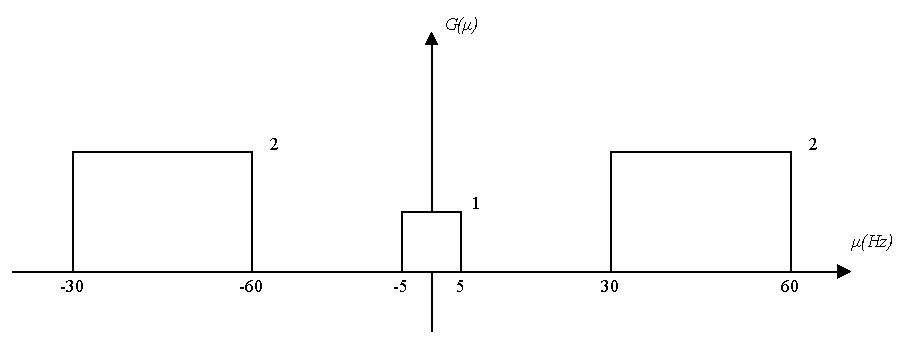
\includegraphics[width=\textwidth]{img/fig_1.pdf}
		\caption{Spettro ideale analitico $G\left(\mu\right)$.}
	\end{figure}

	\noindent
	Descrivere analiticamente in \underline{frequenza} e nel \underline{tempo} il segnale $g\left(t\right)$.\newline
	
	\noindent
	Descrivere inoltre:
	\begin{itemize}
		\item Analiticamente, nel \underline{tempo} e in \underline{frequenza}
		\item Graficamente, in \underline{frequenza}
	\end{itemize}
	Le elaborazioni a cui il segnale $g\left(t\right)$ è sottoposto se ad esso vengono applicate le operazioni schematizzate dal sistema in Figura 2.
	
	\begin{figure}[!htp]
		\centering
		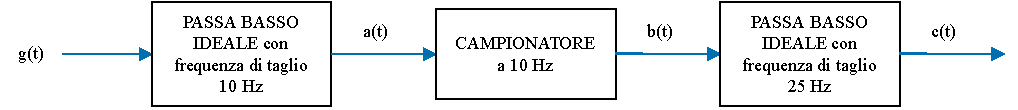
\includegraphics[width=\textwidth]{img/fig_2.pdf}
		\caption{Operazioni da applicare al segnale $g\left(t\right)$.}
	\end{figure}
	
	\section{Esercizio (7 punti)}
	
	Siano $x\left(t\right)$ e $h\left(t\right)$ i due segnali nel dominio continuo del tempo raffigurati in Figura 3.
	
	\begin{figure}[!htp]
		\centering
		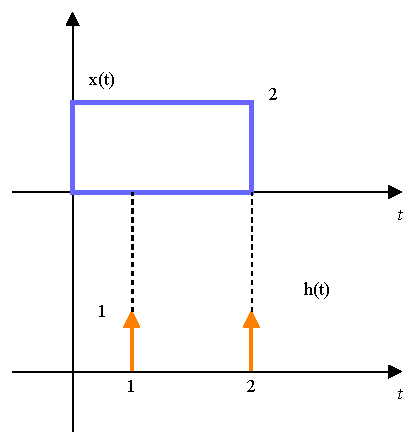
\includegraphics[width=.7\textwidth]{img/fig_3.pdf}
		\caption{Segnali $x\left(t\right)$ e $h\left(t\right)$ nel dominio continuo del tempo.}
	\end{figure}

	\noindent
	Si descriva analiticamente e graficamente il segnale $y\left(t\right)$ ottenuto eseguendo la convoluzione $y\left(t\right) = x\left(t\right) * h\left(t\right)$.
	
	\section{Esercizio (7 punti)}
	
	Si risponda alle seguenti domande:
	\begin{itemize}
		\item Descrivere il fenomeno del \emph{ringing} nell'elaborazione delle immagini. 
		
		\item Spiegare quale algoritmo o filtro dell'elaborazione delle immagini può provocare il \emph{ringing}. Inoltre, fornire una possibile soluzione per eliminare questo fenomeno.
		
		\item Descrivere che cosa è un filtro passa basso ideale. Inoltre, rappresentare un filtro passa bassa ideale, sia graficamente che analiticamente, con frequenze $15$ Hz e $25$ Hz.
	\end{itemize}\newpage
	
	\section{Esercizio (6 punti)}
	
	Il seguente codice, che mira a implementare un'operazione di filtraggio puntuale, contiene un errore semantico.
	\begin{enumerate}
		\item Si indichi dove si trova l'errore e come potrebbe essere corretto.
		\item Si indichi di che operatore si tratta.
	\end{enumerate}
	Si prega di giustificare brevemente le risposte.\newline
	
	\noindent
	NOTA: L'errore potrebbe essere sia sintattico che semantico: con un errore \dquotes{sintattico} il codice non \dquotes{gira} (ad esempio manca una parentesi), con un errore \dquotes{semantico} il codice gira ma non fa quello che dovrebbe fare. Nell'esempio sotto l'errore è semantico, come specificato nel testo dell'esercizio.
	
	\lstinputlisting[language=MATLAB]{code/matlab.mlx}
\end{document}